\chapter{软件分布式共享内存系统与RDMA技术介绍}\label{chap:sdsm}{
    本文研究的基础主要包括软件分布式共享内存系统的实现和远程直接内存访问技术两个方面。因此本章将分别对这两项技术进行系统性阐述,以奠定后续工作的基础。针对软件分布式共享内存系统,首先将介绍其关键技术,然后介绍一些经典和现代软件分布式共享内存示例,重点介绍了国产软件分布式共享内存系统 JIAJIA 的设计与实现;针对 RDMA 技术,将主要介绍其通信原理、RDMA 实现与相关通信库以RDMA通信编程方面的内容。
    \section{软件分布式共享内存关键技术}
    % \begin{figure}[!htbp]
    %     \centering
    %     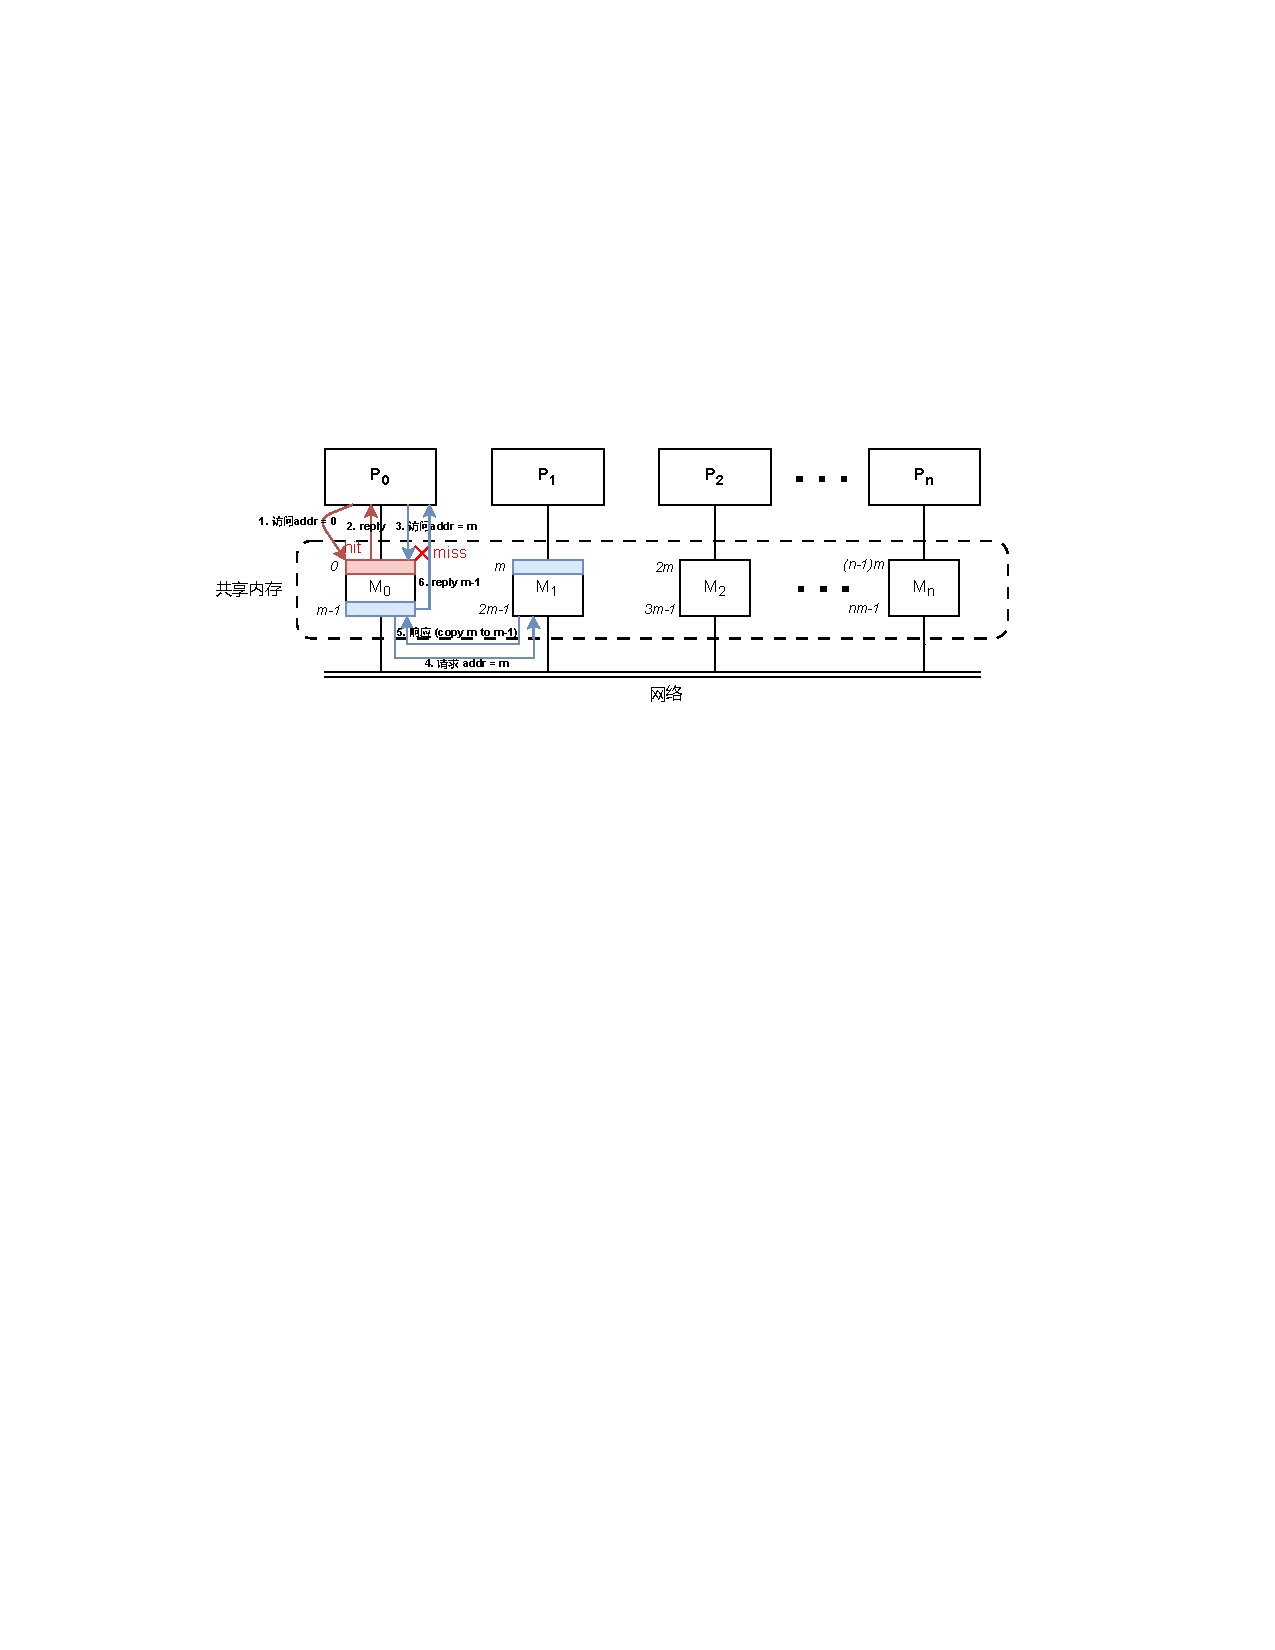
\includegraphics[width=\textwidth]{Img/shared-memory.pdf}
    %     \bicaption{\enspace 软件分布式共享内存}{\enspace shared memory principle}
    %     \label{fig:sharedmemory}
    % \end{figure}

    \subsection{实现层次}\label{sec:implementations}
    软件 DSM 系统实现方式灵活,可以在系统软件(操作系统或编译器)、运行时库、语言等层次上实现。
    \begin{itemize}
        \item \textbf{基于操作系统修改的软件DSM系统}:
              早期的软件 DSM 系统如 IVY\citep{likai1988ivy} ,Munin\citep{bennett1990munin}等通过依赖或修改系统软件来实现共享虚拟内存抽象和一致性管理。
              IVY 通过修改操作系统中的内存管理模块(Memory Management Unit, MMU)来监测远程访问,当处理机访问非本地页时,将触发缺页中断,并由 MMU 向远端取页;
              Munin 建立在 V 内核(V kernel)之上,依赖预处理器来检测用户对共享数据的注释,以便对不同类型的数据执行不同的一致性机制。这些方案由于需要系统软件支持导致可移植性差。

        \item \textbf{基于用户库形式软件 DSM 系统}:
              以用户库形式提供给开发者的全软件 DSM 系统是更为常见的实现。
              通过操作系统接口检测缺页异常并处理。系统初始化时使用 mmap() 建立共享虚拟内存与本地内存的映射,并通过 mprotect() 修改共享页权限。
              越权访问时,操作系统产生段违例信号(SIGSEGV),由预先注册的信号处理程序捕获并完成远程取数和权限授予。
              此类方案完全在用户空间运行,无需修改硬件或系统软件,仅依赖节点间通信能力,可移植性强。典型系统包括 TreadMarks、CRL、OpenSHMEM 及 JIAJIA。

        \item \textbf{基于语言或语言扩展级别的 DSM 系统}:
              语言或语言扩展级别的 DSM 系统在高性能计算社区发展为分区全局地址空间(PGAS)语言,通过扩展现有语言规范提供分布式共享内存编程模型,
              适合 Exascale 规模高性能并行计算。典型代表包括面向 Fortran 的 Coarray Fortran~\citep{numrich1998coarrayfortran, coarryfortran2}、
              面向 Java 的 Titanium~\citep{Yelick1998Titanium}、
              面向 C 的 UPC~\citep{bonachea2013UPC}(Unified Parallel C)以及面向 C++ 的 UPC++~\citep{bachan2019upc++}。
              与传统 DSM 系统的区别在于显式远程数据访问,程序员需明确指定数据来源。实现上依赖编译器和通信中间件层(如 GASNet~\citep{Bonachea2018GASNetEX})支持。
              GASNet 包含核心接口(Core API)和扩展接口(Extended API),前者直接实现于网络架构,后者独立于网络硬件,支持跨网络迁移。
    \end{itemize}

    \begin{figure}
        \centering
        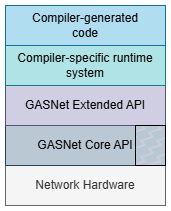
\includegraphics[width=0.3\textwidth]{Img/GASNet.png}
        \bicaption{\enspace GASNet 层系统图}{\enspace GASNet layer disgram}
        \label{fig:GASNET}
    \end{figure}

    \subsection{通信机制}
    软件 DSM 系统依赖底层的消息传递机制来实现上层的虚拟共享抽象。不同网络环境和协议实现的消息传递机制在通信流程和开销上展现出显著差异。

    为了追求更高的性能和可扩展性,传统 DSM 系统通常更倾向于采用低延迟的 UDP。在软件 DSM 系统的典型实现中,通常利用 SIGIO 信号来实现异步I/O通知,当 SIGIO 信号到达时,将导致当前执行被中断,转而执行相应的信号处理程序,之后再恢复原先的执行状态。

    RDMA 网络为现代软件 DSM 系统通信提供双重性能优势。一方面,高带宽、低延迟的特性极大的降低了通信传输延迟;另一方面,通过硬件直接访问内存,绕过内核协议栈,显著降低了协议处理和上下文切换带来的额外延迟。

    \subsection{内存一致性模型}
    内存一致性模型本质上是内存系统与并行程序之间的约定,它限制了系统可以执行内存访问的顺序。不同的内存一致性模型对访问顺序施加的限制的强弱程度不同,具体选择取决于对系统的性能要求和编程复杂度的权衡。维护内存一致性是软件 DSM 系统的关键问题,核心在于何时以及如何传播对共享内存的更新。

    \begin{itemize}
        \item \textbf{严格一致性模型(Strict Consistency):} 严格一致性模型要求任何一次读操作总是返回最近一次对相同对象的写入结果,实现需要全局时钟同步和零通信延迟的理想条件。

        \item \textbf{顺序一致性(Sequential Consistency):} 顺序一致性是最直观的内存一致性模型,最早由 Lamport 形式化定义,要求系统中所有进程对共享数据的操作必须呈现出一个全局的顺序,同时每个进程内部的操作顺序必须与程序中给定的顺序保持一致。

        \item \textbf{处理器一致性(Processor Consistency):} 处理器一致性比顺序一致性弱,核心特性可以概括为以下两条规则:
              \begin{enumerate}[label=\arabic*.]
                  \item 每个处理器内部发出的所有写操作必须以程序中的顺序被其他处理器观察到。
                  \item 对于同一内存地址,所有处理器都必须看到相同的写顺序;对于不同地址的写操作,各处理器可以看到的顺序不完全一致。
              \end{enumerate}

        \item \textbf{TSO(Total Store Order)}是一种特殊的处理器一致性,它通过允许同一处理中后续的读操作可以在写操作完成前提前执行,进一步隐藏了写入延迟,以提升性能。

        \item \textbf{弱一致性(Weak Consistecny):} 弱一致性模型的核心机制在于区分同步操作与普通访存操作,
              开发者通过显式的同步操作保护共享内存的写入,确保多个处理器对同一共享单元的写操作互斥,
              适用于对性能要求较高且数据一致性可容忍一定延迟更新的场景。

              \begin{figure}[!htbp]
                  \centering
                  \begin{subfigure}[b]{0.8\textwidth}
                      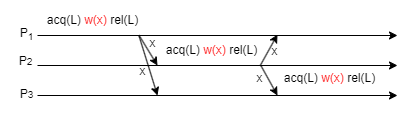
\includegraphics[width=\textwidth]{Img/eager-release-consistency.png}
                      \caption{急切更新释放一致性}
                      \label{fig:eager-release-consistency}
                  \end{subfigure}
                  \\
                  \begin{subfigure}[b]{0.8\textwidth}
                      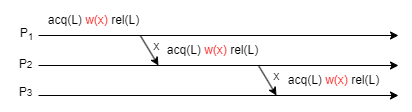
\includegraphics[width=\textwidth]{Img/lazy-release-consistency.png}
                      \caption{懒惰更新释放一致性}
                      \label{fig:lazy-release-consistency}
                  \end{subfigure}

                  \bicaption{\enspace 急切更新释放一致性 vs 懒惰更新释放一致性}{\enspace Eager release consistency vs Lazy release consistency}
                  \label{fig:oaspl}
              \end{figure}

        \item \textbf{释放一致性(Release Consistency):} 释放一致性的核心思想是把弱一致性中的同步操作进一步划分为获取操作(acquire)和释放操作(release)。只在特定的释放操作时才传播对共享内存的更新以保证数据一致性,而不是在每次访问共享内存时都强制同步。

        \item \textbf{懒惰更新释放一致性(Lazy release Consistency):} 懒惰更新释放一致性将更新传播的目的地范围限制为下一个获取锁的节点。这进一步减少了系统中通信消息的数量。
              下图说明懒惰更新释放一致性与急切释放一致性的通信比较。

        \item \textbf{域一致性(Scope Consistency):} 域一致性引入了一致性域(consistency scope)的概念,可以简单地将一致性域视为由锁保护的临界区。
              通过这一概念隐式地建立起共享内存对象与同步对象之间的关联,进而限制每次传播的共享内存对象更新的范围,有效降低了通信数据量。

        \item \textbf{单项一致性(Entry Consistency):} 单项一致性最早由 Midway 系统提出。开发者需要显示建立共享变量与同步变量之间的关联,对每一个共享变量的访问都需要由关联的同步变量来保护。具体而言,当获取同步变量(acquire)时,仅传播与同步变量关联的共享变量的更新。
    \end{itemize}

    \section{软件分布式共享内存系统 JIAJIA}
    \subsection{设计架构}
    \begin{figure}[!htbp]
        \centering
        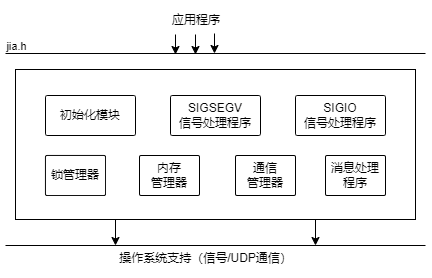
\includegraphics[width=\textwidth]{Img/JIAJIA-design.png}
        \bicaption{\enspace JIAJIA 设计架构}{\enspace JIAJIA design architecture}
        \label{fig:JIAJIA-design}
    \end{figure}
    JIAJIA 是一个国产软件 DSM 系统,以页为共享粒度,在物理分离的内存上提供逻辑共享的虚拟内存。JIAJIA 以用户库的形式提供给开发人员,开发人员可以使用 jia.h 头文件提供的接口编写采用分布式共享内存范式的并行程序,并使用 .jiahosts 配置文件设置参与分布式系统的节点组成。程序运行时,JIAJIA系统将会拷贝应用程序和配置文件到所有参与节点,随后并行执行协同完成任务。图~\ref{fig:JIAJIA-design} 显示了JIAJIA系统所包含的核心模块。

    \begin{enumerate}[label=\arabic*.]
        \item \textbf{初始化模块。}初始化模块用于对整个系统进行准备操作(见图~\ref{fig:JIAJIA-init}),负责加载配置文件(.jiahosts,.jiaconfig)以及初始化各个模块。
              \begin{figure}[!htbp]
                  \centering
                  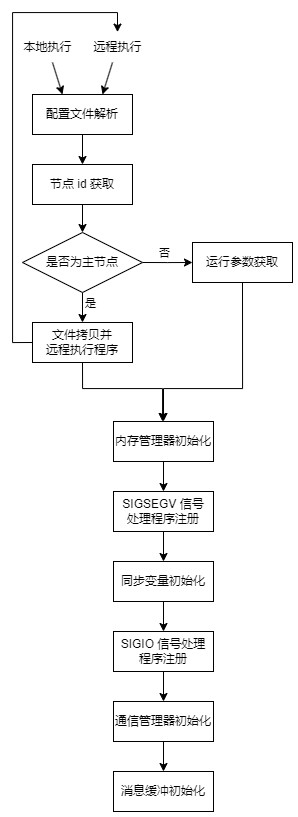
\includegraphics[width=0.6\textwidth]{Img/JIAJIA-init.png}
                  \bicaption{\enspace JIAJIA 初始化模块}{\enspace JIAJIA initialization module}
                  \label{fig:JIAJIA-init}
              \end{figure}

        \item \textbf{内存管理器。} JIAJIA 采用 NUMA 结构,是一个基于宿主(home-based)的系统,每个共享页都有对应的宿主节点核心包含三个数据结构:用于记录本地分配的共享页的目录(home),用于记录缓存页状态的缓存目录(cache),用于记录全部共享页的页目录(page)。JIAJIA 的内存组织如~\ref{fig:JIAJIA-memory}所示。
              \begin{figure}[!htbp]
                  \centering
                  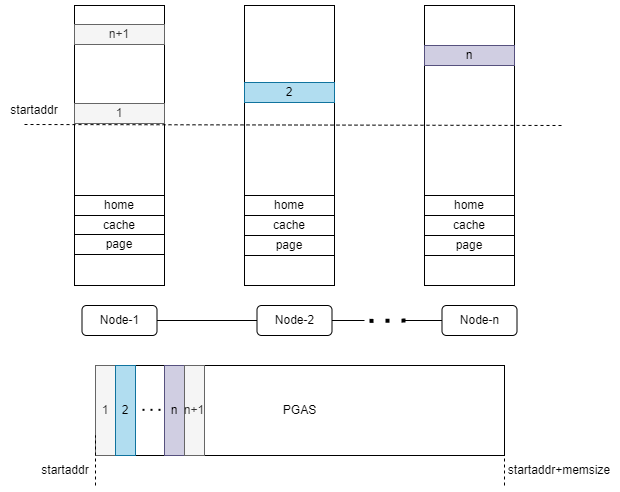
\includegraphics[width=0.65\textwidth]{Img/JIAJIA-memory.png}
                  \bicaption{\enspace JIAJIA 内存组织}{\enspace JIAJIA memory structure}
                  \label{fig:JIAJIA-memory}
              \end{figure}

        \item \textbf{SIGSEGV 信号处理程序。} JIAJIA 系统中任何节点都可以透明地访问任一共享内存位置。这一机理利用了操作系统的信号机制:当应用程序试图访问无权限内存时,将触发段违例信号(SIGSEGV),操作系统将捕获该信号并将其发送给预设的 SIGSEGV 信号处理程序。该程序将完成对本地内存的授权或对远程内存的取页操作。如图~\ref{fig:JIAJIA-access}所示。
              \begin{figure}[!htbp]
                  \centering
                  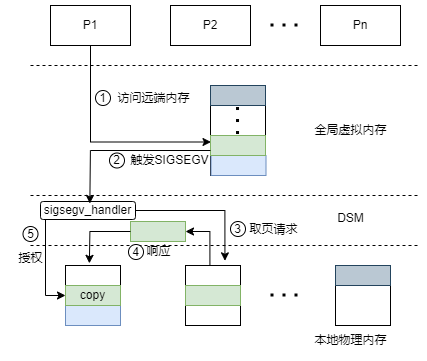
\includegraphics[width=0.65\textwidth]{Img/jiajia-access.png}
                  \bicaption{\enspace JIAJIA 访问远端内存}{\enspace JIAJIA }
                  \label{fig:JIAJIA-access}
              \end{figure}

        \item \textbf{通信管理器。} JIAJIA 使用通信管理器记录并管理发送和接收的套接字描述符。详见~\ref{chap:sdsm:sec:sigio}小节。

        \item \textbf{消息处理程序。} JIAJIA 底层基于消息传递机制,消息处理程序主要负责处理接收到的本地或远程消息,并根据消息类型执行相应的操作。如图~\ref{fig:JIAJIA-message-handle}。图~\ref{fig:JIAJIA-message-types}展示了JIAJIA中存在的消息类型。
              \begin{figure}[!htbp]
                  \centering
                  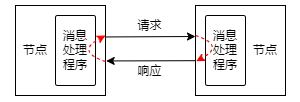
\includegraphics[width=0.50\textwidth]{Img/message-handler.png}
                  \bicaption{\enspace JIAJIA 底层消息传递机制}{\enspace JIAJIA underlying message passing mechanism}
                  \label{fig:JIAJIA-message-handle}
              \end{figure}

              \begin{figure}[!htbp]
                  \centering
                  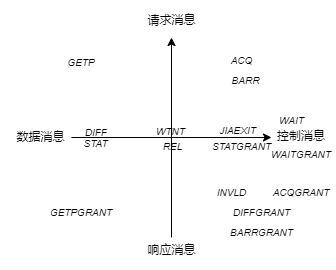
\includegraphics[width=0.50\textwidth]{Img/message-types.png}
                  \bicaption{\enspace JIAJIA 消息类型}{\enspace JIAJIA message types}
                  \label{fig:JIAJIA-message-types}
              \end{figure}

        \item \textbf{锁管理器。} 锁管理器主要负责同步变量的分配管理。JIAJIA 支持两种同步变量:锁(lock)和屏障(barrier)。开发者可以分别通过 jia\_lock 和 jia\_barrier 来请求锁或屏障的授权。对于锁同步变量,锁管理器维护一个先入先出队(FIFO)队列,按请求顺序依次授予锁权限;对于屏障同步变量,锁管理器通过计数器判断所有节点是否抵达相同位置,并在全部到达后统一授予继续运行的权限。
    \end{enumerate}

    \subsection{基于锁的缓存一致性协议}
    在内存一致性模型方面,JIAJIA 采用域一致性模型,并实现了一种基于锁的缓存一致性协议。该协议支持写失效的传播策略,并利用多写协议来避免假共享。

    JIAJIA 使用同步变量将应用程序分割为一个个一致性域(或称为临界区间),每到达一个同步原语都代表一个旧临界区间的结束,以及新临界区间的开始,见图~\ref{fig:JIAJIA-scopes}。
    在旧临界区间(如scope1)结束时,将传播在该临界区中对共享页做的修改给相应的宿主节点。
    JIAJIA 基于锁的一致性协议的特点是它将一个临界区域内对共享页的修改信息(写通知,write-notice)与锁绑定,
    write-notice 记录了修改页的地址,获取锁的处理机将根据锁管理器中的 write-notice 得知哪些页面已被其他处理机修改。
    在处理临界区嵌套情况时,JIAJIA 使用堆栈结构来记录锁的嵌套,获取锁时压栈,释放锁时弹栈,弹栈时将把栈顶锁的 write-notice 合并到下一层。

    \begin{figure}[!htbp]
        \centering
        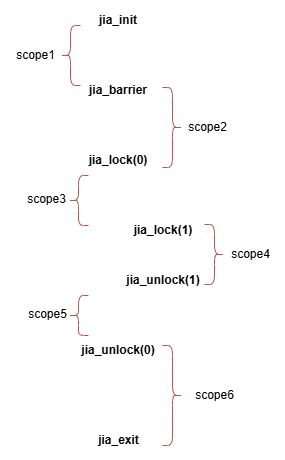
\includegraphics[width=0.50\textwidth]{Img/JIAJIA-scope.png}
        \bicaption{\enspace JIAJIA 一致性域}{\enspace JIAJIA consistency scope}
        \label{fig:JIAJIA-scopes}
    \end{figure}

    \section{RDMA 技术介绍}
    远程直接内存访问(Remote Direct Memory Access, RDMA)技术是一种应用于高性能计算领域的网络通信协议,支持远程直接读写异地内存,而无需双方操作系统甚至 CPU 的介入。
    如图~\ref{fig:DMA-RDMA}所示,RDMA 可视作直接内存访问(Direct Memory Access, DMA)在分布式系统上的扩展,把直接访问内存的范围从单机内存扩展到了远端内存。
    \begin{figure}[!htbp]
        \centering
        \begin{subfigure}[b]{0.40\textwidth}
            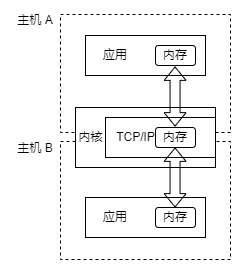
\includegraphics[width=\textwidth]{Img/TCPIP.png}
            \caption{TCP/IP 通信}
            \label{fig:TCPIP}
        \end{subfigure}%
        ~~~~~% add desired spacing
        \begin{subfigure}[b]{0.40\textwidth}
            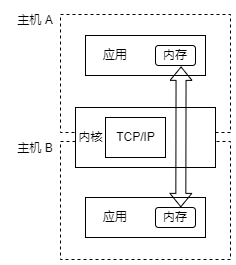
\includegraphics[width=\textwidth]{Img/RDMA.png}
            \caption{RDMA 通信}
            \label{fig:RDMA}
        \end{subfigure}
        \bicaption{\enspace DMA 与 RDMA 的比较}{\enspace }
        \label{fig:DMA-RDMA}
    \end{figure}

    RDMA(Remote Direct Memory Access)是一种针对传统 TCP/IP 网络协议栈(图~\ref{fig:TCPIP})高延迟和高 CPU 开销问题的优化方案。
    在传统的 TCP/IP 通信模式下,跨机器的应用通信需要经历多个数据拷贝过程:
    首先,应用数据需从用户空间拷贝至内核空间,然后由 TCP/IP 协议栈进行封装,接着传输至驱动层,最终写入网卡缓存并发送到远端。
    这一过程中涉及复杂的协议处理和多次数据拷贝,导致 CPU 负担沉重,影响通信效率。

    相比之下,RDMA 通信模式(图~\ref{fig:RDMA})通过硬件直接访问内存,实现数据传输,无需拷贝至内核空间,同时由硬件完成协议处理并将数据传输至远端设备。
    RDMA 主要具备以下三大核心特性:

    \begin{enumerate}[label=\arabic*.]
        \item \textbf{零拷贝}(Zero-Copy)。数据可以直接从发送端用户空间传输到接收端用户空间,无需在内核空间与用户空间之间进行多次拷贝,从而减少延迟,提高吞吐量。
        \item \textbf{内核旁路}(Kernel Bypass)。RDMA 采用用户态驱动(如 Verbs API)直接控制网卡,绕过传统 TCP/IP 协议栈,避免内核态的数据封装、解析及中断处理,从而减少上下文切换的开销。
        \item \textbf{CPU 卸载}(CPU Offloading)。RDMA 通过两种方式降低 CPU 负担:
              \begin{itemize}
                  \item 网络协议处理(如报文组装、分片重组、流量控制等)完全由网卡硬件执行,而非 CPU 处理;
                  \item 采用 RDMA 内存语义(如 RDMA Read/Write)进行数据传输时,远端 CPU 无需参与,从而进一步减少计算资源的占用。
              \end{itemize}
    \end{enumerate}

    \subsection{RDMA 通信模式与通信原语}
    RDMA 使用 QPs 作为通信基本单元行通信,QPs 的类型决定了 RDMA 通信链路的模式。见图~\ref{fig:rdma-queue-pairs}。
    \begin{figure}[!htbp]
        \centering
        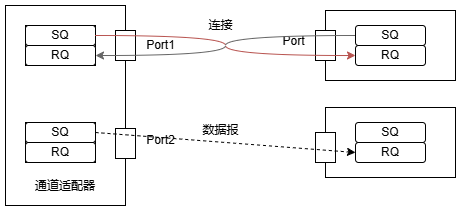
\includegraphics[width=\linewidth]{Img/QueuePairs.png}
        \bicaption{\enspace RDMA 队列对}{\enspace RDMA Queue Pairs}
        \label{fig:rdma-queue-pairs}
    \end{figure}

    QPs 的类型可以根据是否建立连接以及是否可靠来划分。因此 RDMA 相应的支持四种通信链路模式即四种类型的 QPs,分别是:可靠连接(RC)、不可靠连接(UC)、不可靠数据报(UD)、可靠数据报(RD)。其中 RC 模式和 UC 模式均是点对点通信,在通信之前需要在节点之间建立一对一的连接,区别是RC 模式提供可靠的传输服务,而 UC 模式无法确保数据包按序、无丢失交付,可靠性需要由上层协议来保证。UD 模式类似于 UDP ,特点是面向无连接通信、支持多播、以及单个消息大小受限于路径最大传输单元(path MTU)。RD 模式当前并未有实现支持。

    RDMA 支持两类通信原语即所谓的动词(Verbs),双向动词和单向动词。双向动词又称为消息语义,包含 SEND 和 RECV ,适合传输控制消息;单向动词又称为内存语义,包含 RDMA Read 、RDMA Write 和 RDMA 原子操作(Fetch-and-Add/FAA,Compare-and-Swap/CAS),RDMA Read 和 RDMA Write 适合大量数据传输,RDMA 原子操作适合需要强一致性保证和低延迟并发控制的场景。表~\ref{tab:mode-verbs}展示了 RDMA 通信模式和通信原语的支持关系。

    \begin{table}[!htbp]
        \footnotesize% fontsize
        \setlength{\tabcolsep}{4pt}% column separation
        \renewcommand{\arraystretch}{1.5}% row space 
        \centering
        \begin{tabular}{lcccc}
            \hline
            %\multicolumn{num_of_cols_to_merge}{alignment}{contents} \\
            %\cline{i-j}% partial hline from column i to column j
               & Send/Recv  & RDMA Write & RDMA Read  & RDMA Atomic \\
            \hline
            RC & \checkmark & \checkmark & \checkmark & \checkmark  \\
            UC & \checkmark & \checkmark & \times     & \times      \\
            UD & \checkmark & \times     & \times     & \times      \\
            \hline
        \end{tabular}
        \bicaption{\enspace RDMA 通信模式与通信原语的关系}{\enspace Relation between RDMA communication mode and verbs}% caption
        \label{tab:mode-verbs}
    \end{table}

    \subsection{RDMA 通信流程}
    不同的 RDMA Verbs 在通信时有不同的执行的流程,以下是对几种常见 Verbs 通信流程的介绍。
    \begin{enumerate}[label=\arabic*.]
        \item Send/Recv 通信流程

              \begin{figure}[!htbp]
                  \centering
                  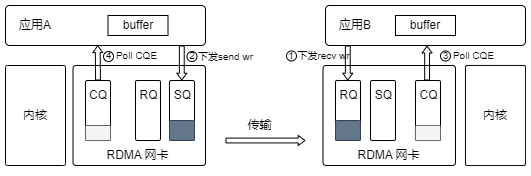
\includegraphics[width=\linewidth]{Img/RDMA-Send.png}
                  \bicaption{\enspace Send/Recv 通信流程图}{\enspace Send/Recv Communication Flow Diagram}
                  \label{fig:rdma-send}
                  {\small Note: 不同 RDMA 实现对于通信硬件设备有不同的名称,本文统称为 RDMA 网卡}
              \end{figure}
              图~\ref{fig:rdma-send}显示了左侧应用A尝试利用 Send 向远程应用 B 发送数据(其中省略了RDMA 网卡访存的操作)的流程。为了实现这一通信,将执行如下步骤:
              \begin{itemize}
                  \item 应用 B 首先向 RQ 下发接收工作请求,其中包含了对 RDMA 网卡的提示,网卡将据此把接收到的数据放到内存中的指定位置。
                  \item 应用 A 向 SQ 中下发发送工作请求,
                        本地网卡将根据 SQE 从应用 A 的内存取出数据并发往远端。
                  \item 远端 RDMA 网卡接收到数据后根据RQ 中的提示将数据放入应用 B 的相应内存中。
                  \item 网卡将请求的执行状态放入 CQ 中,应用可通过轮询得到上一个请求的结果。
              \end{itemize}

              从上述流程中可以看出,Send/Recv 操作需要接收方 CPU 的参与。而且需要注意的是,在不同链路模式下,CQE 产生的时机会有所不同。UD模式下,在将数据放入网络后便产生 CQE;而RC模式下,可能需要等到远端发回确认消息后,才会产生 CQE 。

        \item RDMA Read 通信流程
              \begin{figure}[!htbp]
                  \centering
                  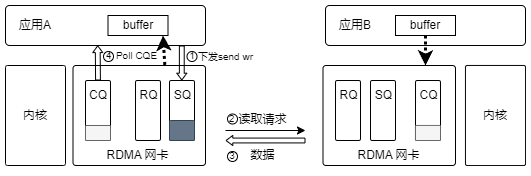
\includegraphics[width=\linewidth]{Img/RDMA-Read.png}
                  \bicaption{\enspace RDMA Read 通信流程图}{\enspace RDMA Read Communication Flow Diagram}
                  \label{fig:rdma-Read}
              \end{figure}

              RDMA Read 用于直接读取远端内存。如~\ref{fig:rdma-Read}所示,其执行流程如下:
              \begin{itemize}
                  \item 应用 A 向 SQ 中下发读取工作请求。
                  \item 本地网卡根据 SQ 中的 WQE 向远端发送读取请求包。
                  \item 远端网卡接收到读取请求包后,根据包中携带的信息,读取应用 B 相应位置的内存,并发回数据。
                  \item 本地网卡接收到数据,根据 WQE 的信息将数据存入应用 A 的内存,并向 CQ 中存入CQE。
                  \item 应用通过轮询 CQ 获得 CQE,从中获取上一个请求的完成情况。
              \end{itemize}

        \item RDMA Write 通信流程
              \begin{figure}[!htbp]
                  \centering
                  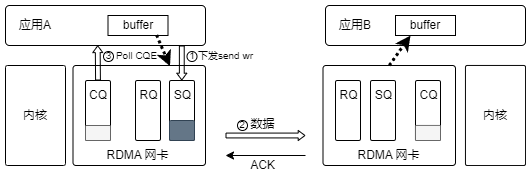
\includegraphics[width=\linewidth]{Img/RDMA-Write.png}
                  \bicaption{\enspace RDMA Write 通信流程图}{\enspace RDMA Write Communication Flow Diagram}
                  \label{fig:rdma-Write}
              \end{figure}

              RDMA Write 用于直接写入远端内存。如~\ref{fig:rdma-Write}所示,其执行流程如下:
              \begin{itemize}
                  \item 应用 A 向 SQ 中下发写入工作请求。
                  \item 本地网卡根据 SQ 中的 WQE 中的提示读取本地内存,组装数据包发往远端。
                  \item 远端网卡收到数据包后解析得到数据目的地址,将数据写入相应位置后返回 ACK 。
                  \item 本地网卡根据返回的 ACK 信息生成 CQE,并将其放入 CQ。
                  \item 应用通过轮询 CQ 获得 CQE,从中获取上一个请求的完成情况。
              \end{itemize}
    \end{enumerate}

    通过上述的流程分析可得出 RDMA Verbs 的如下特征,双向动词 Send/Recv 需要远端 CPU 参与提前下发接收请求,类似于传统的消息传递模型,而单向动词 RDMA Read、RDMA Write 可以绕过远端CPU,直接读取或写入指定的内存位置。
    无论是 Send 还是 RDMA Read、RDMA Write 都将向 SQ 中下发发送工作请求,网卡将根据其中指定的操作码(Opcode)字段来区分,RQ 仅在 Send/Recv 时使用。相比于RDMA Read, Send/Recv 和 RDMA Write 不需要网卡发回数据包,因此在传输小数据报时,RDMA Write 和 Send/Recv 的传输延迟大约是 RDMA Read 的一半~\citep{kalia2014herd}(见图~\ref{fig:RDMA-Verbs-Latency})。
    \begin{figure}[!htbp]
        \centering
        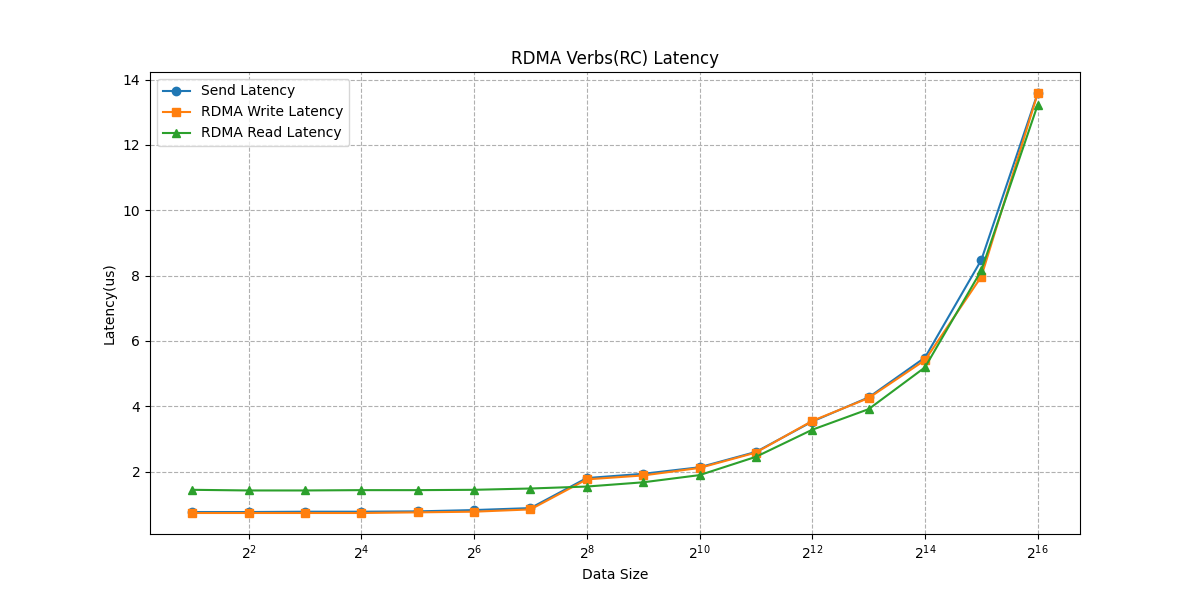
\includegraphics[width=\linewidth]{Img/verbs-latency.png}
        \bicaption{\enspace RDMA Verbs 通信延迟比较}{\enspace Comparison of Communication Latency of RDMA Verbs}
        {\small Note: 在Mellanox ConnectX-3 Pro 网卡可靠连接下的测试}
        \label{fig:RDMA-Verbs-Latency}
    \end{figure}

    \subsection{RDMA 实现与通信基础库}
    \textbf{RDMA 实现架构}:RDMA 有多种不同的实现架构,包括无限带宽(InfiniBand,IB)、基于融合以太网的RDMA(RDMA over Converged Ethernet,RoCE)、互联网广域 RDMA 协议(internet Wide Area RDMA Protocol,iWARP)等。它们之间的区别如图~\ref{fig:RDMA-Implementations}所示:
    \begin{figure}[!htbp]
        \centering
        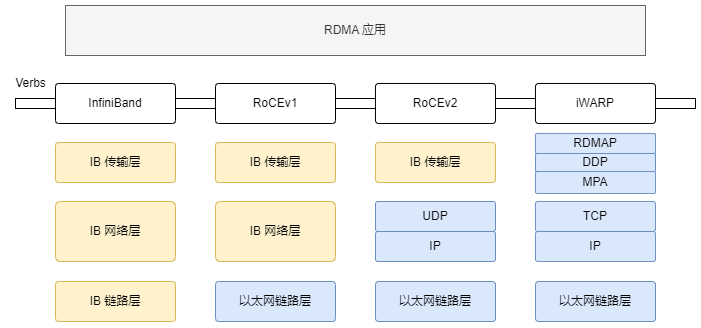
\includegraphics[width=\linewidth]{Img/RDMA-Implementation.png}
        \bicaption{\enspace RDMA 不同实现架构}{\enspace Different RDMA Implementation Architectures}
        \label{fig:RDMA-Implementations}
    \end{figure}

    \begin{enumerate}[label=\arabic*.]
        \item InfiniBand 是由InfiniBand 贸易协会(IBTA)定义的用于高性能计算网络通信标准,其设计目标在于为大规模并行计算系统提供超低延迟和高带宽的数据传输解决方案。该技术采用分层协议结构,通过采用独立于TCP/IP 的全新网络协议栈,有效规避了操作系统协议栈带来的性能损耗。在物理层实现上,IB 网络构建需要专用硬件基础设施,包括IB 交换机、IB 路由器,以及配置了Host Channel Adapter(HCA)的终端节点。这些架构特性使其在支持 RDMA 上展现出显著性能优势,目前在超级计算机集群、分布式存储系统以及人工智能训练平台等对网络性能要求严苛的场景下被广泛应用。
        \item RoCE 同样是由 IBTA 提出的在以太网上支持RDMA的协议,其核心目标是通过复用传统以太网硬件设施以降低 RDMA 技术的部署成本。目前包含两个版本RoCEv1和RoCEv2。RoCEv1 在以太网链路层(L2)实现了IB 传输层数据包的封装,通过以太网帧直接承载远程内存访问操作。但由于未引入IP层路由机制,其通信范围被限制在单一广播域内,仅支持同一子网或VLAN内的节点间数据传输,且需依赖无损以太网的优先级流量控制(PFC)技术以规避丢包风险。RoCEv2 通过利用UDP/IP协议栈封装IB传输层数据,即保留了 IB 传输层语义又增加了对路由功能的支持,从而突破RoCEv1 对子网的边界限制,使其成为更大规模部署的通用解决方案。
        \item iWARP 是互联网工程任务组(IETF)提出的在TCP/IP协议栈上实现远程直接内存访问(RDMA)的技术体系。该技术基于三层核心组件——从上层向下层依次是远程直接内存访问协议(Remote Direct Memory Access Protocol, RDMAP)、直接数据放置(Direct Data Placement, DDP)和标记协议数据单元对齐(Marker PDU Aligned Framing, MPA)。其中 RDMAP 负责提供零拷贝操作原语,DDP 解耦网络传输与内存语义映射,MPA负责保证 TCP 报文边界对齐。 由于 TCP 是面向连接的,iWARP 仅支持点对点可靠通信,缺乏对组播和广播的支持。
    \end{enumerate}

    上述三种不同的 RDMA 实现,由于在协议栈设计、硬件依赖及端到端传输机制等方面的不同,在性能、成本和扩展性上也存在差异。性能上,IB \text{>} RoCEv2 \text{>} iWARP(由高到低);部署成本上,iWARP \text{>} RoCEv2 \text{>} IB(由低到高);可扩展性上,iWARP \text{>} RoCEv2 \text{>} IB(由高到低);不过RDMA 网卡厂商为了应对异构网络环境,通常会通过灵活设计的硬件架构同时支持两种不同的架构,比如英伟达(NVIDIA)的ConnectX系列网卡兼容IB和RoCEv2双模式,而掣速科技(Chelsio)的T6系列网卡则同时支持 RoCEv2 和 iWARP。

    \textbf{RDMA 通信基础库}: 为了开发可以原生利用 RDMA 的应用,OpenFabrics 联盟推动实现了一组协议无关的统一软件编程接口,用户利用这些接口可以开发出在 IB、RoCE、iWARP架构上无缝移植的应用。其中通信传输方面涉及到两个核心用户空间库,\textbf{libibverbs} 和 \textbf{librdmacm}。
    % \begin{enumerate}[label=\arabic*.]
    %     \item \textbf{libibverbs} 是InfiniBand Verbs API的底层实现库,提供了对RDMA硬件的直接访问能力。核心功能包括设备操作、通信管理(QP管理,任务下发)、内存注册、完成处理等。
    %         \begin{table}[!htbp]
    %             \footnotesize% fontsize
    %             \setlength{\tabcolsep}{4pt}% column separation
    %             \renewcommand{\arraystretch}{1.5}% row space 
    %             \centering
    %             \begin{tabular}{|p{1.3cm}|p{4.5cm}|p{5.5cm}|p{3.7cm}|}
    %                 \hline
    %                 %\multicolumn{num_of_cols_to_merge}{alignment}{contents} \\
    %                 %\cline{i-j}% partial hline from column i to column j
    %                  & 准备 & 使用 & 销毁\\
    %                  \hline
    %                  \multirow{2}{*}{设备操作} &   ibv\_get\_device\_list, & ibv\_query\_device, ibv\_query\_port, & ibv\_close\_device \\
    %                  & ibv\_open\_device & ibv\_query\_gid, ibv\_query\_pkey & \\
    %                 \hline
    %                通信管理 & ibv\_create\_qp, ibv\_open\_qp & ibv\_post\_recv, ibv\_post\_send & ibv\_destroy\_qp \\
    %                 \hline
    %                 内存注册 & ibv\_alloc\_pd, ibv\_reg\_mr &  & ibv\_dealloc\_pd, ibv\_dereg\_mr \\
    %                 \hline
    %                 \multirow{2}{*}{完成处理} & ibv\_create\_cq, & ibv\_poll\_cq, ibv\_req\_notify\_cq, & ibv\_destroy\_cq, \\
    %                 & ibv\_create\_comp\_channel  & ibv\_get\_cq\_event, ibv\_ack\_cq\_events & ibv\_destroy\_comp\_channel \\
    %                 \hline
    %             \end{tabular}
    %             \bicaption{\enspace libibverbs 库核心接口}{\enspace libibverbs core API}% caption
    %             \label{tab:libibverbs-api}
    %         \end{table}    
    %     \item \textbf{librdmacm} 是一个 RDMA 通信管理库,为建立 RDMA 连接提供类似 Socket 的编程抽象,并对部分 libibverbs 的接口进行了包装。核心功能包括连接管理、事件处理、资源管理等。
    %         \begin{table}[!htbp]
    %             \footnotesize% fontsize
    %             \setlength{\tabcolsep}{4pt}% column separation
    %             \renewcommand{\arraystretch}{1.5}% row space 
    %             \centering
    %             \begin{tabular}{|p{1.3cm}|p{4.5cm}|p{5.5cm}|p{3.7cm}|}
    %                 \hline
    %                 %\multicolumn{num_of_cols_to_merge}{alignment}{contents} \\
    %                 %\cline{i-j}% partial hline from column i to column j
    %                  & 准备 & 使用 & 销毁\\
    %                  \hline
    %                  \multirow{7}{*}{连接管理} &   rdma\_create\_event\_channel, & 
    %                  rdma\_get\_cm\_event, rdma\_ack\_cm\_event  & rdma\_destroy\_event\_channel \\
    %                  &  & rdma\_event\_str  & \\
    %                  & rdma\_create\_id & rdma\_resolve\_addr, rdma\_resolve\_route  & rdma\_destroy\_id \\
    %                  &  & rdma\_connect, rdma\_disconnect  & \\
    %                  &  & rdma\_bind\_addr, rdma\_listen  & \\
    %                  &  & rdma\_accept, rdma\_reject  & \\
    %                 &  & rdma\_migrate\_id  & \\
    %                 \hline
    %                 \multirow{4}{*}{资源管理} & rdma\_create\_ep, rdma\_create\_qp & rdma\_post\_send, rdma\_post\_recv, & rdma\_destroy\_ep, \\
    %                 & rdma\_reg\_msgs & rdma\_post\_read, rdma\_post\_write & rdma\_destroy\_qp \\
    %                 &rdma\_reg\_read, rdma\_reg\_write & ... & \\
    %                 \hline
    %             \end{tabular}
    %             \bicaption{\enspace librdmacm 库核心接口}{\enspace librdmacm core API}% caption
    %             \label{tab:compiler}
    %         \end{table}   
    % \end{enumerate}

    \subsection{RDMA 通信 vs Socket 通信}
    套接字(Socket)API 是传统网络通信的核心编程接口,为TCP/IP协议栈提供了标准化的进程间通信机制。该接口通过抽象通信端点实现了跨主机的数据传输能力,每个套接字由本地IP地址与端口号组成的二元组唯一标识,并与对端地址共同构成完整的通信链路。在 UNIX/Linux 系统上,套接字是一类特殊的文件,通过文件描述符机制与其他输入/输出(I/O)资源共享相同的接口。这种设计遵循 "一切皆文件" 的哲学,使得网络通信可以像文件读写一样进行操作,例如可以使用 read、write系统调用来接收和发送数据。此外,文件描述符的多路复用技术(如 select、poll 和 epoll)同样可以用于同时管理多个套接字,以提高 I/O 处理的效率。

    根据传输层协议差异,套接字主要分为三种类型:基于TCP协议的流式套接字(stream socket)、基于UDP协议的数据报套接字(datagram socket)和绕过传输层的原始套接字(raw socket),见图~\ref{fig:Socket-Type}。
    \begin{figure}[!htbp]
        \centering
        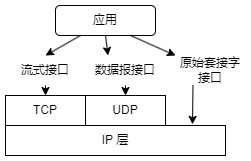
\includegraphics[width=0.35\linewidth]{Img/Socket-Type.png}
        \bicaption{\enspace 三种 Socket 类型}{\enspace The Three Socket Types}
        \label{fig:Socket-Type}
    \end{figure}
    在传统网络编程实践中,传输层协议的选择不仅决定socket的类型,还深刻影响整个通信子系统的设计,主要体现在连接管理、数据传输、错误处理等方面,这里对使用TCP/UDP两种最常用的传输层协议进行了比较。

    \begin{itemize}
        \item 连接管理:TCP是面向连接的协议,在数据传输前需要通过三次握手完成客户端和服务器的建连,客户端将使用 connect() 主动发起连接,而服务器需要调用 listen() 提前进入监听状态并调用 accept() 处理客户端连接,在通信结束双方使用 close() 断连;而 UDP 是无连接协议,无需建立和维护连接,应用程序可直接使用 sendto() 和 recvfrom() 进行通信。
        \item 数据传输:TCP采用字节流的方式传输数据,提供可靠、有序的数据传递;而 UDP采用数据报的形式进行传输,通过 sendto()/recvfrom() 对完成一个数据包的发送和接收。
        \item 错误处理:TCP 协议采用滑动窗口、超时重传和流量控制机制确保数据的可靠交付;而 UDP 传输的可靠性需要依赖应用层的确认和重传机制。
    \end{itemize}

    相比之下,RDMA 通信需要开发者深入了解底层网络协议与硬件特性。通信流程如下(以可靠连接为例):
    \begin{enumerate}[label=\textbf{步骤 \arabic*.}, leftmargin=0.5cm, align=left]
        \item \textbf{设备发现与初始化}
              \begin{itemize}
                  \item 通过\texttt{ibv\_get\_device\_list()}获取网卡设备列表,选择使用的设备(ibv\_device)。
                  \item 通过\texttt{ibv\_open\_device()}打开指定设备,获取设备上下文(ibv\_context)。
              \end{itemize}

        \item \textbf{资源隔离域构建与内存注册}
              \begin{itemize}
                  \item 通过\texttt{ibv\_alloc\_pd()}创建保护域以隔离RDMA资源(ibv\_pd)。
                  \item 通过\texttt{ibv\_reg\_mr()} 注册内存区域(ibv\_mr)。
              \end{itemize}

        \item \textbf{通信终端创建}
              \begin{itemize}
                  \item 通过\texttt{ibv\_create\_cq()}创建完成队列(ibv\_cq)。
                  \item 配置QP属性,并通过\texttt{ibv\_create\_qp()}创建QP(ibv\_qp)。
              \end{itemize}

        \item \textbf{连接建立操作}
              \begin{itemize}
                  \item 可选择采用传统Socket交换通信元数据,或采用 RDMA CM 建连。
              \end{itemize}

        \item \textbf{数据平面操作}
              \begin{itemize}
                  \item 构造工作请求,并指定选用的RDMA操作类型。
                  \item 通过\texttt{ibv\_post\_send()}提交工作请求至发送队列,
                  \item 轮询完成队列并获取完成事件,检验事件状态以判断请求完成情况
              \end{itemize}

        \item \textbf{资源回收操作}
              \begin{itemize}
                  \item 按拓扑逆序销毁队列对、完成队列、内存区域等对象。
                  \item 释放保护域并关闭设备。
              \end{itemize}
    \end{enumerate}
    图~\ref{fig:RDMA-structs}展示了 libibverbs 和 librdmacm 库核心数据结构之间的引用关系。在创建一个数据结构之前,需要首先完成其引用数据结构的创建。
    \begin{figure}[!htbp]
        \centering
        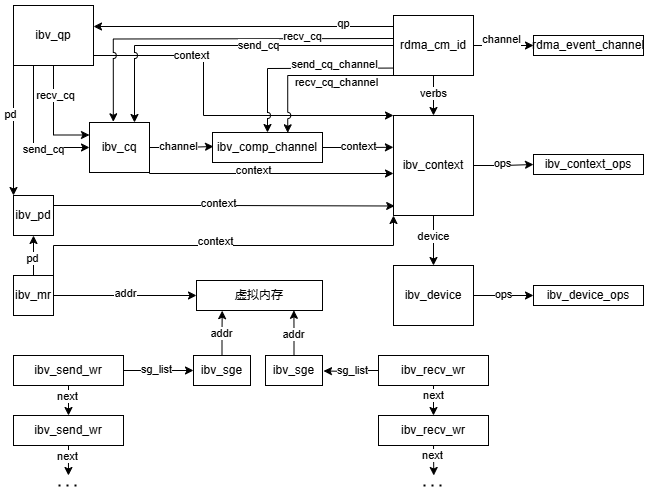
\includegraphics[width=\linewidth]{Img/RDMA-structs.png}
        \bicaption{\enspace RDMA 关键数据结构引用关系图}{\enspace The RDMA key data structure reference relationship diagram}
        \label{fig:RDMA-structs}
    \end{figure}



    \section{本章小结}
}